\documentclass{beamer}

\usepackage[utf8]{inputenc}
\usepackage[spanish]{babel}
\usepackage{amsmath}
\usepackage{amssymb}
\usepackage{tikz}
\usetikzlibrary{arrows,calc,positioning}
%\usetheme{Goddard}
\usetheme{Madrid}
\hypersetup{colorlinks,allcolors=.,urlcolor=magenta}
\usepackage{listings}
\lstset{
    language=Matlab,
    basicstyle=\ttfamily\footnotesize,
    breaklines=true,
    frame=single,
    columns=flexible
}

\title{Investigación de Operaciones II}
\subtitle{Unidad 3: Fundamentos de la Teoría de Colas}
\author[RL]{Ricardo Jesús Largaespada Fernández}
\institute[UNI]{Ingeniería de Sistemas, DACTIC, UNI}
\date{06 de Mayo, 2025}

\begin{document}

% ---------------------------------------------------------------
% TÍTULO Y AGENDA
% ---------------------------------------------------------------
\frame{\titlepage}

\begin{frame}{Agenda}
    \tableofcontents
\end{frame}

\section{Sesión 17}

\begin{frame}{Sesión 17}
\textbf{Tema:}
\begin{enumerate}
    \item Papel de la distribución exponencial.  
\item Proceso de Nacimiento y muerte.
\end{enumerate}

\textbf{Objetivo:}
\begin{itemize}
    \item Comprender el papel de la distribución exponencial en el modelado de tiempos entre llegadas y de servicio, así como los fundamentos del proceso de nacimiento y muerte, para aplicarlos en el análisis cuantitativo de sistemas de colas y la evaluación de su desempeño en contextos reales.
\end{itemize}
\end{frame}

\begin{frame}
\frametitle{Distribución Exponencial}
\framesubtitle{Definición}

En los modelos de colas, los tiempos entre llegadas y servicios suelen modelarse con una \textbf{distribución exponencial}, definida por:
\[
f(t) = \lambda e^{-\lambda t}, \quad t > 0
\]

\begin{itemize}
    \item $\lambda$ representa la tasa promedio de ocurrencia de eventos.
    \item $t$ es el tiempo transcurrido entre eventos sucesivos.
\end{itemize}
\end{frame}

\begin{frame}
\frametitle{Distribución Exponencial}
\framesubtitle{Propiedades Matemáticas}

\begin{itemize}
    \item \textbf{Valor esperado:}
    \[
    E\{t\} = \frac{1}{\lambda}
    \]

    \item \textbf{Probabilidad acumulada:}
    \[
    P\{t \leq T\} = \int_0^T \lambda e^{-\lambda t} dt = 1 - e^{-\lambda T}
    \]
\end{itemize}
\end{frame}

\begin{frame}
\frametitle{Aleatoriedad en los Modelos de Colas}
\framesubtitle{Fenómeno Totalmente Aleatorio}

\begin{itemize}
    \item La ocurrencia de un evento (como una llegada o un servicio) es \textbf{independiente del tiempo transcurrido} desde el último evento.
    \item Esta propiedad se conoce como \textbf{falta de memoria} de la distribución exponencial.
    \item Ejemplo:
    \begin{itemize}
        \item Si la última llegada fue a las 8:02 a.m., y ahora son las 8:20 a.m., la probabilidad de una nueva llegada antes de las 8:29 a.m. depende solo del intervalo (9 minutos), no de la hora previa.
    \end{itemize}
\end{itemize}
\end{frame}

\begin{frame}
\frametitle{Propiedad de Olvido}
\framesubtitle{Falta de Memoria de la Distribución Exponencial}

\begin{itemize}
    \item La distribución exponencial tiene la \textbf{propiedad de olvido} o \textbf{falta de memoria}.
    \item Si $S$ es el tiempo desde el último evento, entonces:
    \[
    P\{t > T + S \mid t > S\} = P\{t > T\}
    \]
    \item Es decir, la probabilidad de esperar más tiempo no depende del tiempo ya esperado.
\end{itemize}
\end{frame}

\begin{frame}
\frametitle{Verificación de la Propiedad de Olvido}
\framesubtitle{Demostración Matemática}

Para la distribución exponencial con media $\frac{1}{\lambda}$:

\[
P\{t > Y\} = 1 - P\{t < Y\} = e^{-\lambda Y}
\]

\[
P\{t > T + S \mid t > S\} = \frac{P\{t > T + S\}}{P\{t > S\}} = 
\frac{e^{-\lambda (T + S)}}{e^{-\lambda S}} = e^{-\lambda T} = P\{t > T\}
\]

\begin{itemize}
    \item Esto confirma la propiedad de que el proceso no tiene memoria.
\end{itemize}
\end{frame}

\begin{frame}
\frametitle{Ejemplo: Fallas en un Sistema de TI}
\framesubtitle{Modelo de Fallas con Distribución Exponencial}

Un sistema de respaldo se activa de inmediato si el servidor principal falla. El tiempo entre fallas del sistema sigue una distribución exponencial con una media de 5 horas.

\vspace{0.3cm}
El administrador del sistema afirma que “el servidor principal suele fallar alrededor de las 8:30 p.m.” todos los días.

\begin{itemize}
    \item Tasa de fallas: $\lambda = \frac{1}{5} = 0.2$ fallas por hora.
    \item Distribución del tiempo entre fallas:
    \[
    f(t) = 0.2 e^{-0.2t}, \quad t > 0
    \]
\end{itemize}
\end{frame}

\begin{frame}
\frametitle{Ejemplo: Fallas en un Sistema de TI}
\framesubtitle{Análisis de la Afirmación del Administrador}

El tiempo entre fallas en sistemas críticos se modela como un proceso aleatorio. La afirmación de una “hora típica de falla” contradice la propiedad de \textbf{falta de memoria} de la distribución exponencial.

\begin{itemize}
    \item Si ahora son las 8:30 p.m., la probabilidad de una falla en los próximos 10 minutos es:
    \[
    P\left\{t < \frac{10}{60} \right\} = 1 - e^{-0.2 \left(\frac{10}{60}\right)} = 0.03278
    \]
    
    \item Si son la 1:00 p.m., la probabilidad de una falla hacia las 8:30 p.m. se incrementa a aproximadamente 0.777.

    \item Estos resultados muestran que las fallas no siguen patrones diarios fijos, sino que ocurren de forma aleatoria.
\end{itemize}
\end{frame}

\begin{frame}
\frametitle{Modelos de Nacimiento y Muerte Puros}
\framesubtitle{Definición y Aplicaciones}

\begin{itemize}
    \item El modelo de \textbf{nacimiento puro} considera solo llegadas. Ejemplo: creación de registros de nacimiento.
    \item El modelo de \textbf{muerte pura} considera solo salidas. Ejemplo: retiro aleatorio de artículos en inventario.
    \item Ambos modelos son útiles en análisis de sistemas donde se modela el cambio en el número de elementos (clientes, ítems, procesos).
\end{itemize}
\end{frame}

\begin{frame}
\frametitle{Distribuciones en los Modelos}
\framesubtitle{Relación entre Exponencial y Poisson}

\begin{itemize}
    \item En estos modelos:
    \begin{itemize}
        \item La \textbf{distribución exponencial} describe el tiempo entre eventos (llegadas o salidas).
        \item La \textbf{distribución de Poisson} modela el número de eventos en un intervalo de tiempo fijo.
    \end{itemize}
    
    \item Existe una relación directa entre ambas: 
    \begin{itemize}
        \item Si los tiempos entre eventos son exponenciales, entonces el conteo de eventos sigue una distribución de Poisson.
    \end{itemize}
\end{itemize}
\end{frame}

\begin{frame}
\frametitle{Modelo de Nacimiento Puro}
\framesubtitle{Definición y Fundamento}

\begin{itemize}
    \item Se modela la llegada de eventos (clientes, solicitudes, etc.) en el tiempo.
    \item Sea $p_0(t)$ la probabilidad de que no haya llegadas en el intervalo $t$.
    \item Dado que el tiempo entre llegadas es exponencial:
    \[
    p_0(t) = P\{\text{tiempo entre llegadas} \geq t\} = e^{-\lambda t}
    \]
    \item Para $h \to 0$:
    \[
    p_0(h) \approx 1 - \lambda h
    \quad \Rightarrow \quad
    p_1(h) = 1 - p_0(h) \approx \lambda h
    \]
\end{itemize}
\end{frame}

\begin{frame}
\frametitle{Modelo de Nacimiento Puro}
\framesubtitle{Ecuaciones Diferenciales y Distribución de Poisson}

\begin{itemize}
    \item Sea $p_n(t)$ la probabilidad de $n$ llegadas en tiempo $t$.
    \item Para $h$ pequeño:
    \[
    p_n(t + h) \approx p_n(t)(1 - \lambda h) + p_{n-1}(t)\lambda h, \quad n > 0
    \]
    \[
    p_0(t + h) \approx p_0(t)(1 - \lambda h)
    \]
    \item Derivando:
    \[
    p_n'(t) = -\lambda p_n(t) + \lambda p_{n-1}(t), \quad n > 0
    \]
    \[
    p_0'(t) = -\lambda p_0(t)
    \]
\end{itemize}
\end{frame}

\begin{frame}
\frametitle{Modelo de Nacimiento Puro}
\framesubtitle{Balance de probabilidades y Ecuaciones diferenciales}

\begin{block}{1. Balance en un intervalo pequeño \(h\)}
Estado \(n\to n\): no llega nadie en \([t,t+h]\)
    \[
      p_n(t)\times P(0\text{ llegadas en }h)
      \;\approx\;p_n(t)\,(1-\lambda h).
    \]
Estado \(n-1\to n\): llega exactamente uno
    \[
      p_{n-1}(t)\times P(1\text{ llegada en }h)
      \;\approx\;p_{n-1}(t)\,\lambda h.
    \]
Descartamos \(\ge2\) llegadas porque son \(o(h)\). Por tanto, para \(n>0\):
    \[
      p_n(t+h)\approx p_n(t)\,(1-\lambda h)
      +p_{n-1}(t)\,\lambda h.
    \]
  \item Para \(n=0\) sólo cabe “quedarse en cero”:
    \[
      p_0(t+h)\approx p_0(t)\,(1-\lambda h).
    \]
\end{block}
\end{frame}

\begin{frame}
\frametitle{Modelo de Nacimiento Puro}
\framesubtitle{Balance de probabilidades y Ecuaciones diferenciales}
\begin{block}{2. De diferencia a derivada}
\[
\frac{p_n(t+h)-p_n(t)}{h}
\;\xrightarrow[h\to0]{}\;
p_n'(t)
\,=\,
-\lambda\,p_n(t)
\;+\;\lambda\,p_{n-1}(t),
\quad n>0,
\]
\[
p_0'(t)=-\lambda\,p_0(t).
\]
\begin{itemize}
  \item El término \(-\lambda p_n\) es la “fuga” desde \(n\).
  \item El término \(+\lambda p_{n-1}\) es el “flujo” que entra en \(n\).
\end{itemize}
\end{block}

\begin{block}{3. Solución: distribución de Poisson}
Con condiciones iniciales
\(
  p_0(0)=1,\;p_n(0)=0\;(n>0)
\),
se obtiene
\[
  p_n(t)
  = \frac{(\lambda t)^n}{n!}\,e^{-\lambda t},
\]
es decir, \(N(t)\sim\mathrm{Poisson}(\lambda t)\).
\end{block}
\end{frame}

\begin{frame}
\frametitle{Solución del Modelo}
\framesubtitle{Distribución de Poisson}

La solución del sistema de ecuaciones diferenciales es:

\[
p_n(t) = \frac{(\lambda t)^n e^{-\lambda t}}{n!}, \quad n = 0, 1, 2, \dots
\]

\begin{itemize}
    \item Esto es una \textbf{distribución de Poisson} con media $E[n|t] = \lambda t$.
    \item Relación clave:
    \begin{itemize}
        \item Tiempo entre llegadas $\sim$ exponencial $\Rightarrow$ número de llegadas $\sim$ Poisson.
    \end{itemize}
\end{itemize}
\end{frame}

\begin{frame}
\frametitle{Resumen: Relación Exponencial–Poisson}
\framesubtitle{Comparación de Distribuciones}

\begin{center}
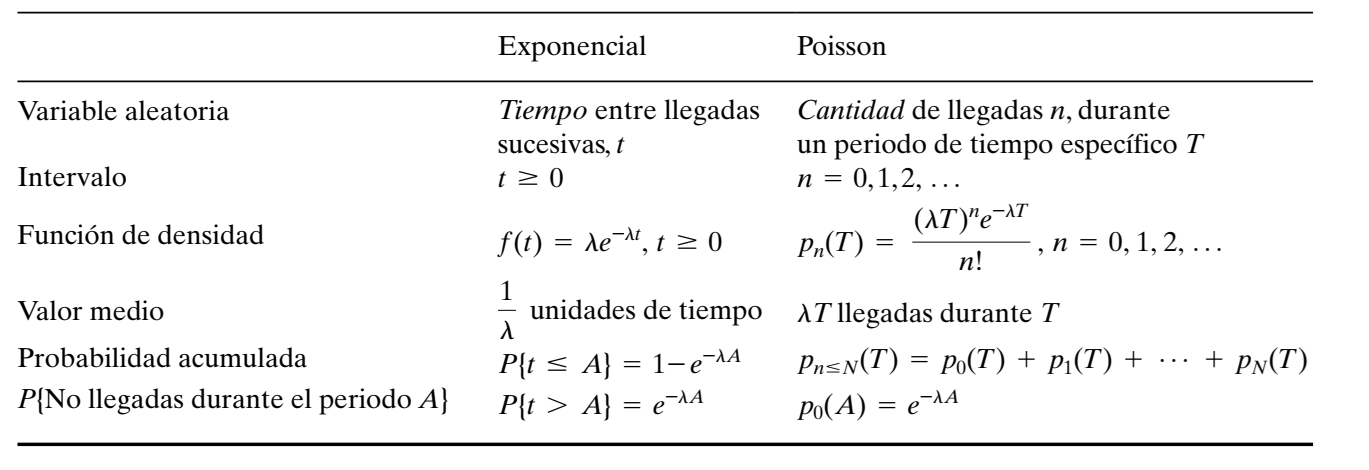
\includegraphics[scale=0.5]{images/tabla.png}
\end{center}
\end{frame}

\begin{frame}
\frametitle{Ejemplo: Nacimientos en una Ciudad}
\framesubtitle{Datos y objetivos}

En una ciudad grande nacen bebés a razón de uno cada 12 minutos. El tiempo entre nacimientos sigue una distribución exponencial.

\vspace{0.2cm}
Determine lo siguiente:

\begin{enumerate}
    \item Cantidad promedio de nacimientos por año.
    \item Probabilidad de que no ocurran nacimientos durante 1 día.
    \item Probabilidad de registrar 50 nacimientos en 3 horas, dado que hubo 40 en las primeras 2.
\end{enumerate}
\end{frame}

\begin{frame}
\frametitle{Ejemplo: Nacimientos en una Ciudad}
\framesubtitle{Parte (a) — Promedio de nacimientos}

\begin{itemize}
    \item Tasa por hora:
    \[
    \lambda = \frac{60}{12} = 5 \text{ nacimientos/hora}
    \]
    \item Por día:
    \[
    \lambda = 24 \times 5 = 120 \text{ nacimientos/día}
    \]
    \item Por año:
    \[
    \lambda t = 120 \times 365 = 43{,}800 \text{ nacimientos/año}
    \]
\end{itemize}
\end{frame}

\begin{frame}
\frametitle{Ejemplo: Nacimientos en una Ciudad}
\framesubtitle{Parte (b) — Probabilidad de 0 nacimientos en 1 día}

\begin{itemize}
    \item Usamos la distribución de Poisson:
    \[
    p_0(1) = \frac{(120)^0 e^{-120}}{0!} = e^{-120} \approx 0
    \]

    \item Alternativamente, usando la distribución exponencial:
    \[
    P\{t > 1 \text{ día}\} = e^{-120} \approx 0
    \]

    \item Interpretación: es prácticamente imposible que no ocurra un nacimiento en un día.
\end{itemize}
\end{frame}

\begin{frame}
\frametitle{Ejemplo: Nacimientos en una Ciudad}
\framesubtitle{Parte (c) — Condicional con distribución de Poisson}

\begin{itemize}
    \item En 3 horas se registraron 50 nacimientos, 40 en las primeras 2 horas.
    \item Quedan 10 nacimientos en la última hora:
    \[
    p_{10}(1) = \frac{5^{10} e^{-5}}{10!} \approx 0.01813
    \]

    \item La tasa usada es:
    \[
    \lambda = \frac{60}{12} = 5 \text{ nacimientos/hora}
    \]
    \item Es decir, hay una probabilidad baja de que justo 10 nacimientos ocurrieran en esa última hora.
\end{itemize}
\end{frame}

\begin{frame}
\frametitle{Modelo de Muerte Pura}
\framesubtitle{Definición del Modelo}

\begin{itemize}
    \item El sistema comienza con $N$ clientes en $t = 0$.
    \item No se permiten nuevas llegadas.
    \item Las salidas ocurren aleatoriamente a una tasa de $\mu$ clientes por unidad de tiempo.
    \item Interés: $p_n(t)$ = probabilidad de que $n$ clientes permanezcan después de tiempo $t$.
\end{itemize}
\end{frame}

\begin{frame}
\frametitle{Modelo de Muerte Pura}
\framesubtitle{Ecuaciones Diferenciales}

\begin{itemize}
    \item A partir del desarrollo para $h$ pequeño:
    \[
    p_N(t + h) = p_N(t)(1 - \mu h)
    \]
    \[
    p_n(t + h) = p_n(t)(1 - \mu h) + p_{n+1}(t)\mu h, \quad 0 < n < N
    \]
    \[
    p_0(t + h) = p_0(t)(1) + p_1(t)\mu h
    \]

    \item Derivando al tomar $h \to 0$:
    \[
    p_N'(t) = -\mu p_N(t)
    \]
    \[
    p_n'(t) = -\mu p_n(t) + \mu p_{n+1}(t), \quad 0 < n < N
    \]
    \[
    p_0'(t) = \mu p_1(t)
    \]
\end{itemize}
\end{frame}

% ------------------- Frame 1 -------------------
\begin{frame}
\frametitle{Modelo de Muerte Pura}
\framesubtitle{Balance de probabilidades en un intervalo $h$ pequeño}

\begin{itemize}
  \item Partimos de que en cada estado sólo “muere” (se va) como máximo una unidad en $h$, pues dos o más muertes son de orden $o(h)$.
  \medskip
  \item Estado tope \(N\to N\):  
    Si había \(N\) individuos, para permanecer en \(N\) nadie puede morir en $h$:
    \[
      p_N(t+h)
      = p_N(t)\times P(0\text{ muertes en }h)
      \;\approx\; p_N(t)\,(1-\mu\,h).
    \]
  \medskip
  \item Estado intermedio \(n\to n\) ó \(n+1\to n\):  
  \begin{itemize}
    \item Quedarse en \(n\): \(p_n(t)\,(1-\mu h)\).  
    \item Venir de \(n+1\): \(p_{n+1}(t)\times P(1\text{ muerte en }h)\approx p_{n+1}(t)\,\mu h\).
  \end{itemize}
    \[
      p_n(t+h)
      \approx p_n(t)\,(1-\mu h)
      \;+\;
      p_{n+1}(t)\,\mu h,
      \quad 0<n<N.
    \]
  \medskip
  \item Estado \(0\to0\):  
    No puede morir nadie, pero puede llegar desde 1:
    \[
      p_0(t+h)
      = p_0(t)\,(1)
      + p_1(t)\,\mu h.
    \]
\end{itemize}
\end{frame}

% ------------------- Frame 2 -------------------
\begin{frame}
\frametitle{Modelo de Muerte Pura}
\framesubtitle{Ecuaciones diferenciales (Kolmogorov hacia adelante)}

\begin{itemize}
  \item Dividimos por \(h\), restamos \(p(t)\) y tomamos límite \(h\to0\):
  \[
    \frac{p_i(t+h)-p_i(t)}{h}\;\xrightarrow[h\to0]{}\;p_i'(t).
  \]
  \medskip
  \item Para \(n=N\):  
    \[
      p_N'(t)
      = -\mu\,p_N(t).
    \]
  \medskip
  \item Para \(0<n<N\):  
    \[
      p_n'(t)
      = -\mu\,p_n(t)
      \;+\;\mu\,p_{n+1}(t).
    \]
    - \(-\mu p_n\): “fuga” de probabilidad si muere uno y se va a \(n-1\).  
    - \(+\mu p_{n+1}\): “flujo” que llega desde \(n+1\).
  \medskip
  \item Para \(n=0\):  
    \[
      p_0'(t)
      = \mu\,p_1(t),
    \]
    pues el único modo de entrar en 0 es que muera alguien cuando había 1.
\end{itemize}
\end{frame}


\begin{frame}
\frametitle{Modelo de Muerte Pura}
\framesubtitle{Distribución de Poisson Truncada}

\begin{itemize}
    \item La solución del sistema anterior lleva a una distribución de \textbf{Poisson truncada}:
    \[
    p_n(t) = \frac{(\mu t)^{N - n} e^{-\mu t}}{(N - n)!}, \quad n = 1, 2, \dots, N
    \]
    \[
    p_0(t) = 1 - \sum_{n = 1}^{N} p_n(t)
    \]

    \item Describe cómo decae el número de clientes con el tiempo sin llegadas nuevas.
\end{itemize}
\end{frame}

\begin{frame}
\frametitle{Ejemplo: Inventario de Rosas en una Florería}
\framesubtitle{Descripción del problema}

\begin{itemize}
    \item Cada semana se inician con 18 docenas de rosas.
    \item La demanda diaria sigue una \textbf{distribución de Poisson} con media $\mu = 3$ docenas/día.
    \item Se hace un pedido si el inventario baja a 5 docenas o menos.
    \item Las rosas sobrantes al final de la semana se desechan.
\end{itemize}

Queremos determinar:
\begin{enumerate}
    \item Probabilidad de colocar un pedido en un día cualquiera.
    \item Promedio de rosas desechadas al final de la semana.
\end{enumerate}
\end{frame}

\begin{frame}
\frametitle{Ejemplo: Inventario de Rosas}
\framesubtitle{Parte (a) — Probabilidad de colocar un pedido}

Para el día $t$, se coloca un pedido si hay $\leq 5$ docenas:

\[
P_{n \leq 5}(t) = \sum_{n = 0}^{5} p_n(t)
\]

Donde $p_n(t)$ sigue una distribución de Poisson truncada:

\[
p_n(t) = \frac{(3t)^{18 - n} e^{-3t}}{(18 - n)!}
\]

Se calcula para $t = 1, 2, \dots, 7$.
\end{frame}

\begin{frame}
\frametitle{Ejemplo: Inventario de Rosas}
\framesubtitle{Resultados Parte (a)}

\begin{center}
\begin{tabular}{|c|c|c|}
\hline
\textbf{Día (t)} & $\mu t$ & $P_{n \leq 5}(t)$ \\
\hline
1 & 3  & 0.0000 \\
2 & 6  & 0.0088 \\
3 & 9  & 0.1242 \\
4 & 12 & 0.4240 \\
5 & 15 & 0.7324 \\
6 & 18 & 0.9083 \\
7 & 21 & 0.9755 \\
\hline
\end{tabular}
\end{center}

\textbf{Interpretación:} A medida que transcurre la semana, aumenta la probabilidad de que el inventario baje a 5 docenas.
\end{frame}

\begin{frame}
\frametitle{Ejemplo: Inventario de Rosas}
\framesubtitle{Parte (b) — Rosas desechadas al final de la semana}

Queremos calcular el número esperado de docenas restantes al final de la semana $(t = 7)$:

\[
E[n \mid t = 7] = \sum_{n = 0}^{18} n \cdot p_n(7)
\]

\textbf{Resultado:} $E[n \mid t = 7] \approx 0.664$

\textbf{Interpretación:} En promedio se desecha alrededor de \textbf{una docena} de rosas al final de la semana.
\end{frame}


\end{document}
